%%%%%% CMB-S4 Simulations and Data Analysis Chapter  %%%%%%%%%%%%%%%%
 
\chapter{Simulations and Data Analysis}
\renewcommand*\thesection{\arabic{section}}

%%%%%%%%%%%%%%%%%%%%%%%%%%%%%%%%%%%%%%%%%%%%%%%%%%%%%%%%%%%
%%%%%%%%%%%%%%%%%%%%%%%%%%%%%%%%%%%%%%%%%%%%%%%%%%%%%%%%%%%
%%%%%%%%%%%%%%%%%%%%%%%%%%%%%%%%%%%%%%%%%%%%%%%%%%%%%%%%%%%
%%%%%%%%%%%%%%%%%%%%%%%%%%%%%%%%%%%%%%%%%%%%%%%%%%%%%%%%%%%

\section{Introduction}

Overview of simulations and data analysis elements motivating the subsequent division into 5 blocks.

\subsection{Data Analysis}

A sequence of S/N enhancing data compressions via domain transformations - time samples (red) to sky pixels (blue) to map multipoles (green) to physical parameters (yellow).

An iterative process, with each domain exposing different systematic effects to be mitigated.

A full analysis requires propogating not just the data but also their covariance between domains. The size of the full pixel covariance now precludes exact methods except in certain special cases.

\begin{figure}[htbp]
\hspace*{3in}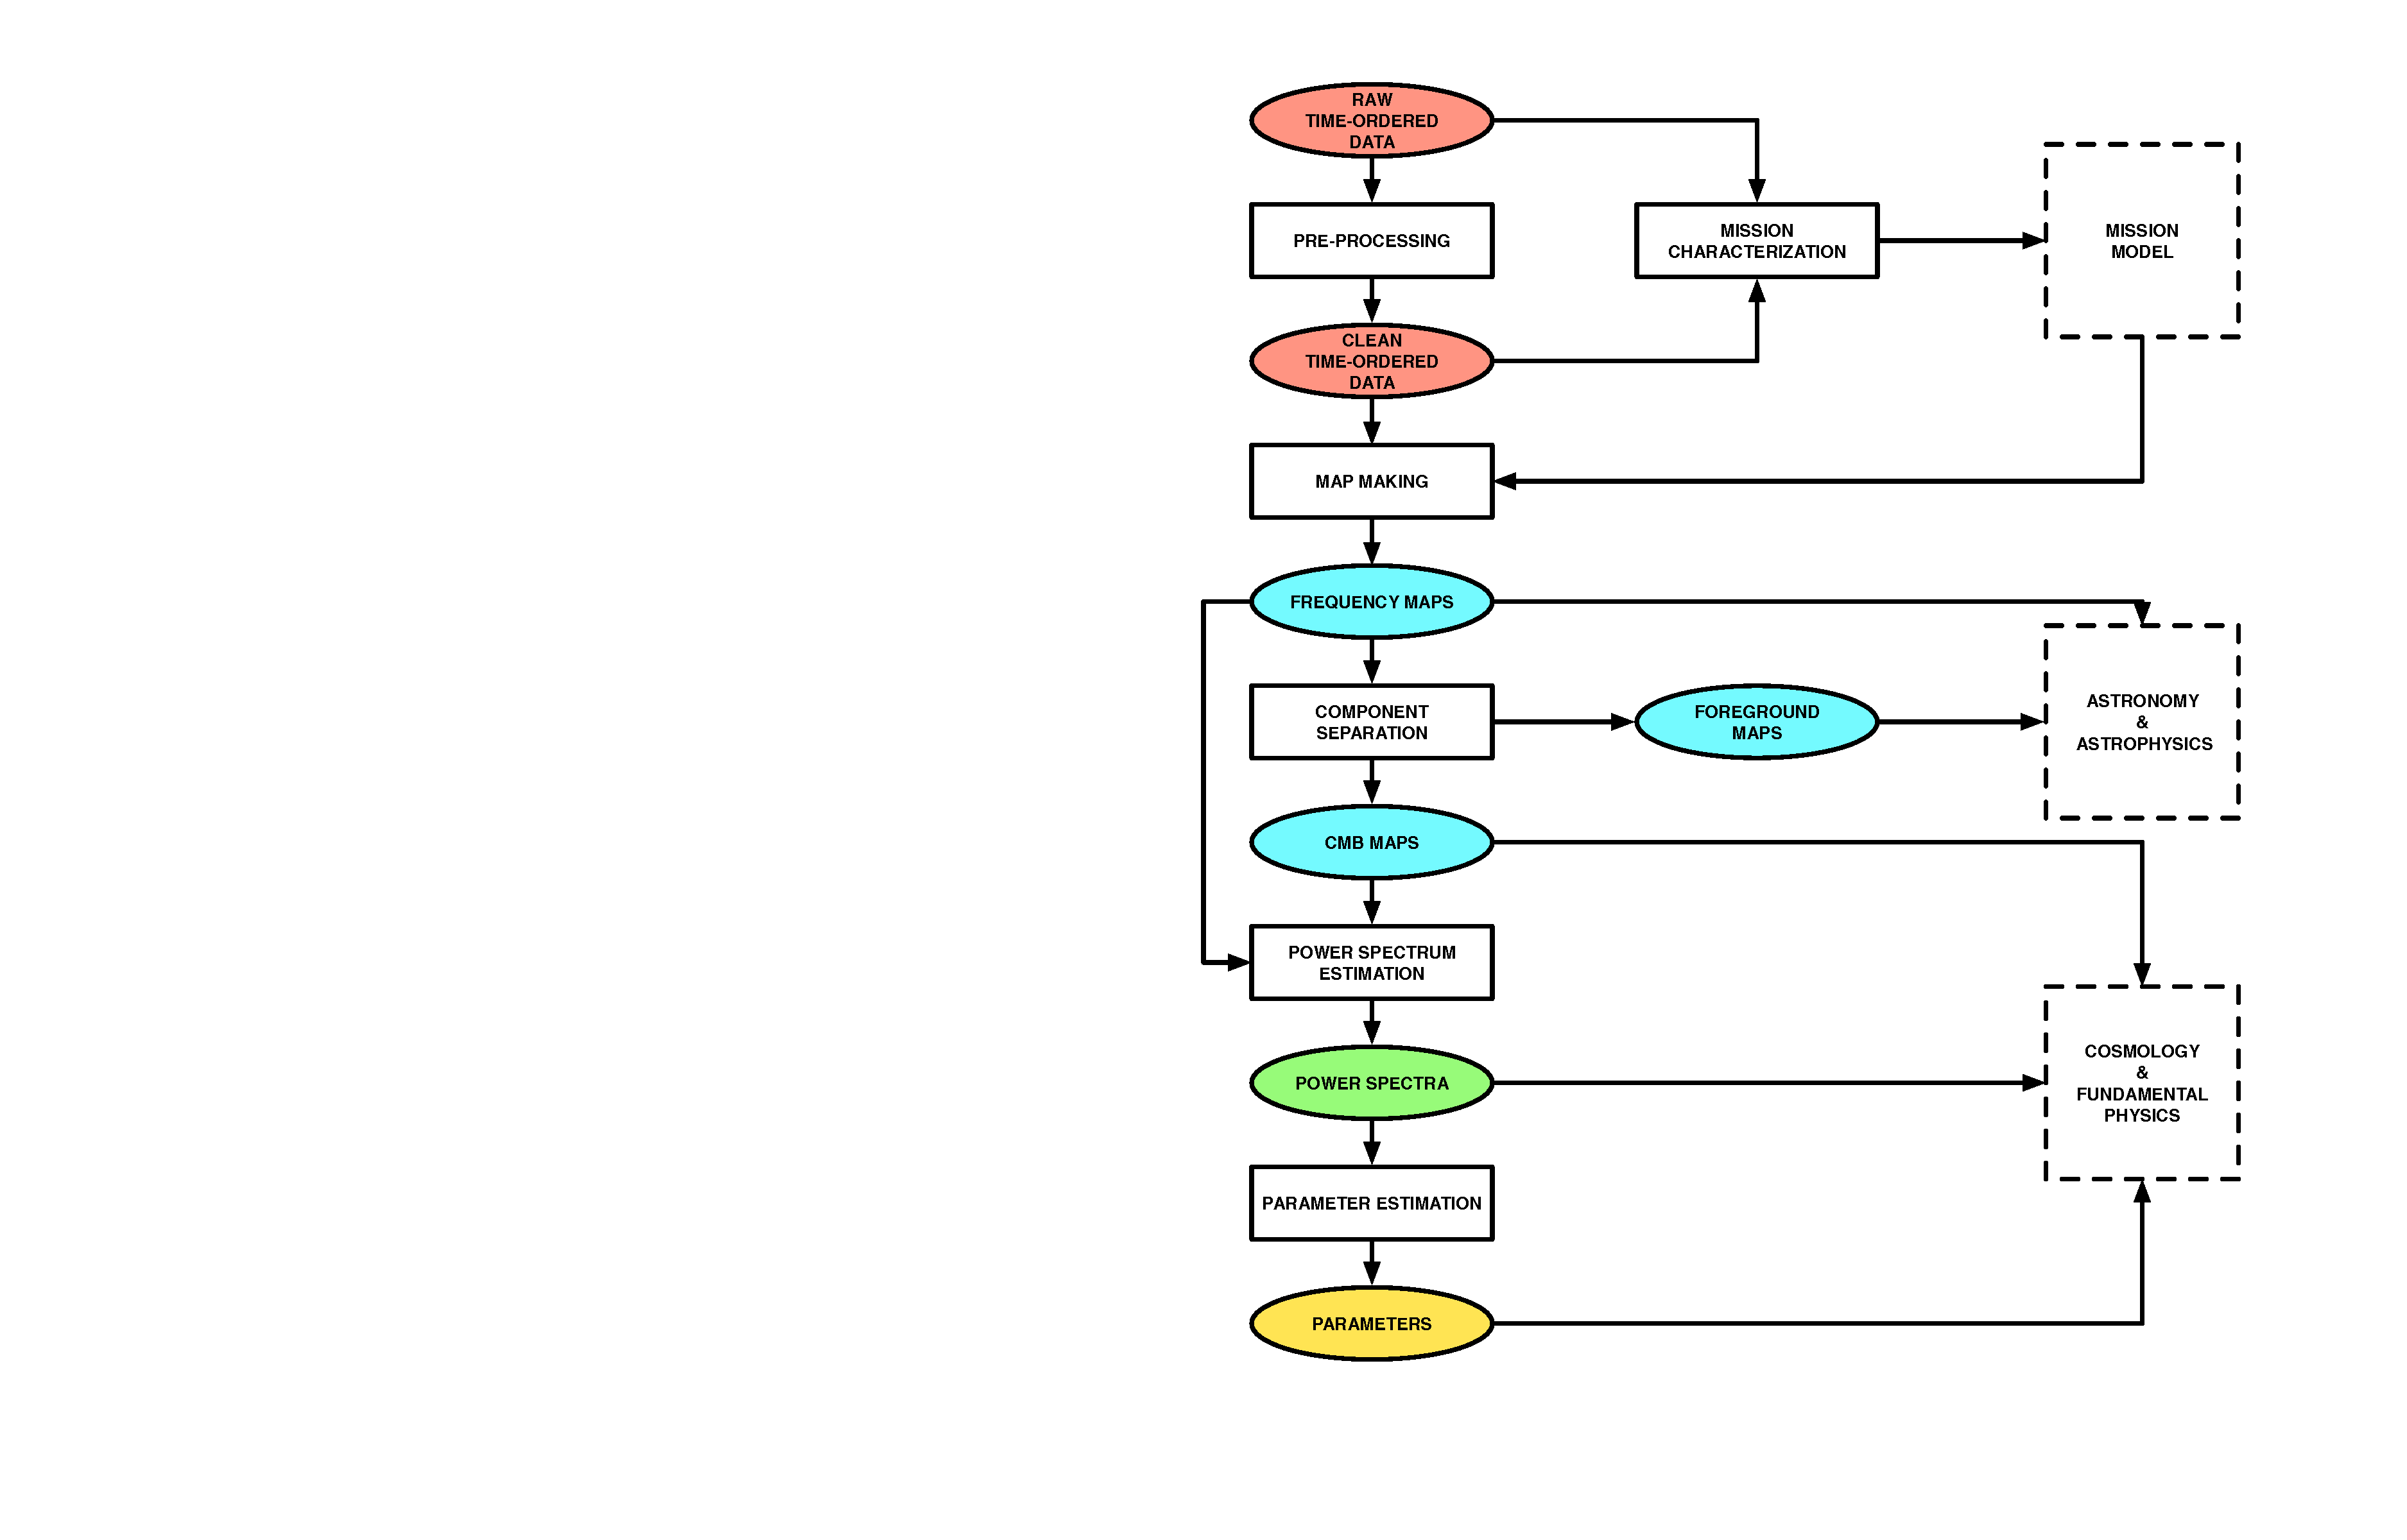
\includegraphics[width=0.5\textwidth]{Analysis/da}
\caption{The CMB data analysis pipeline}
\label{default}

\end{figure}

\newpage

\subsection{Simulation}

Needed for 
\begin{itemize}
\item Mission design and development (both instrument and observation)
\item Validation and verification of analysis tools
\item Absent a full covariance matrix, Monte Carlo based uncertainty quantification and debiasing.
\end{itemize}

From top to bottom, there is an inevitable trade-off between the computational cost of generating the simulation and its realism and accuracy.

\begin{figure}[htbp]
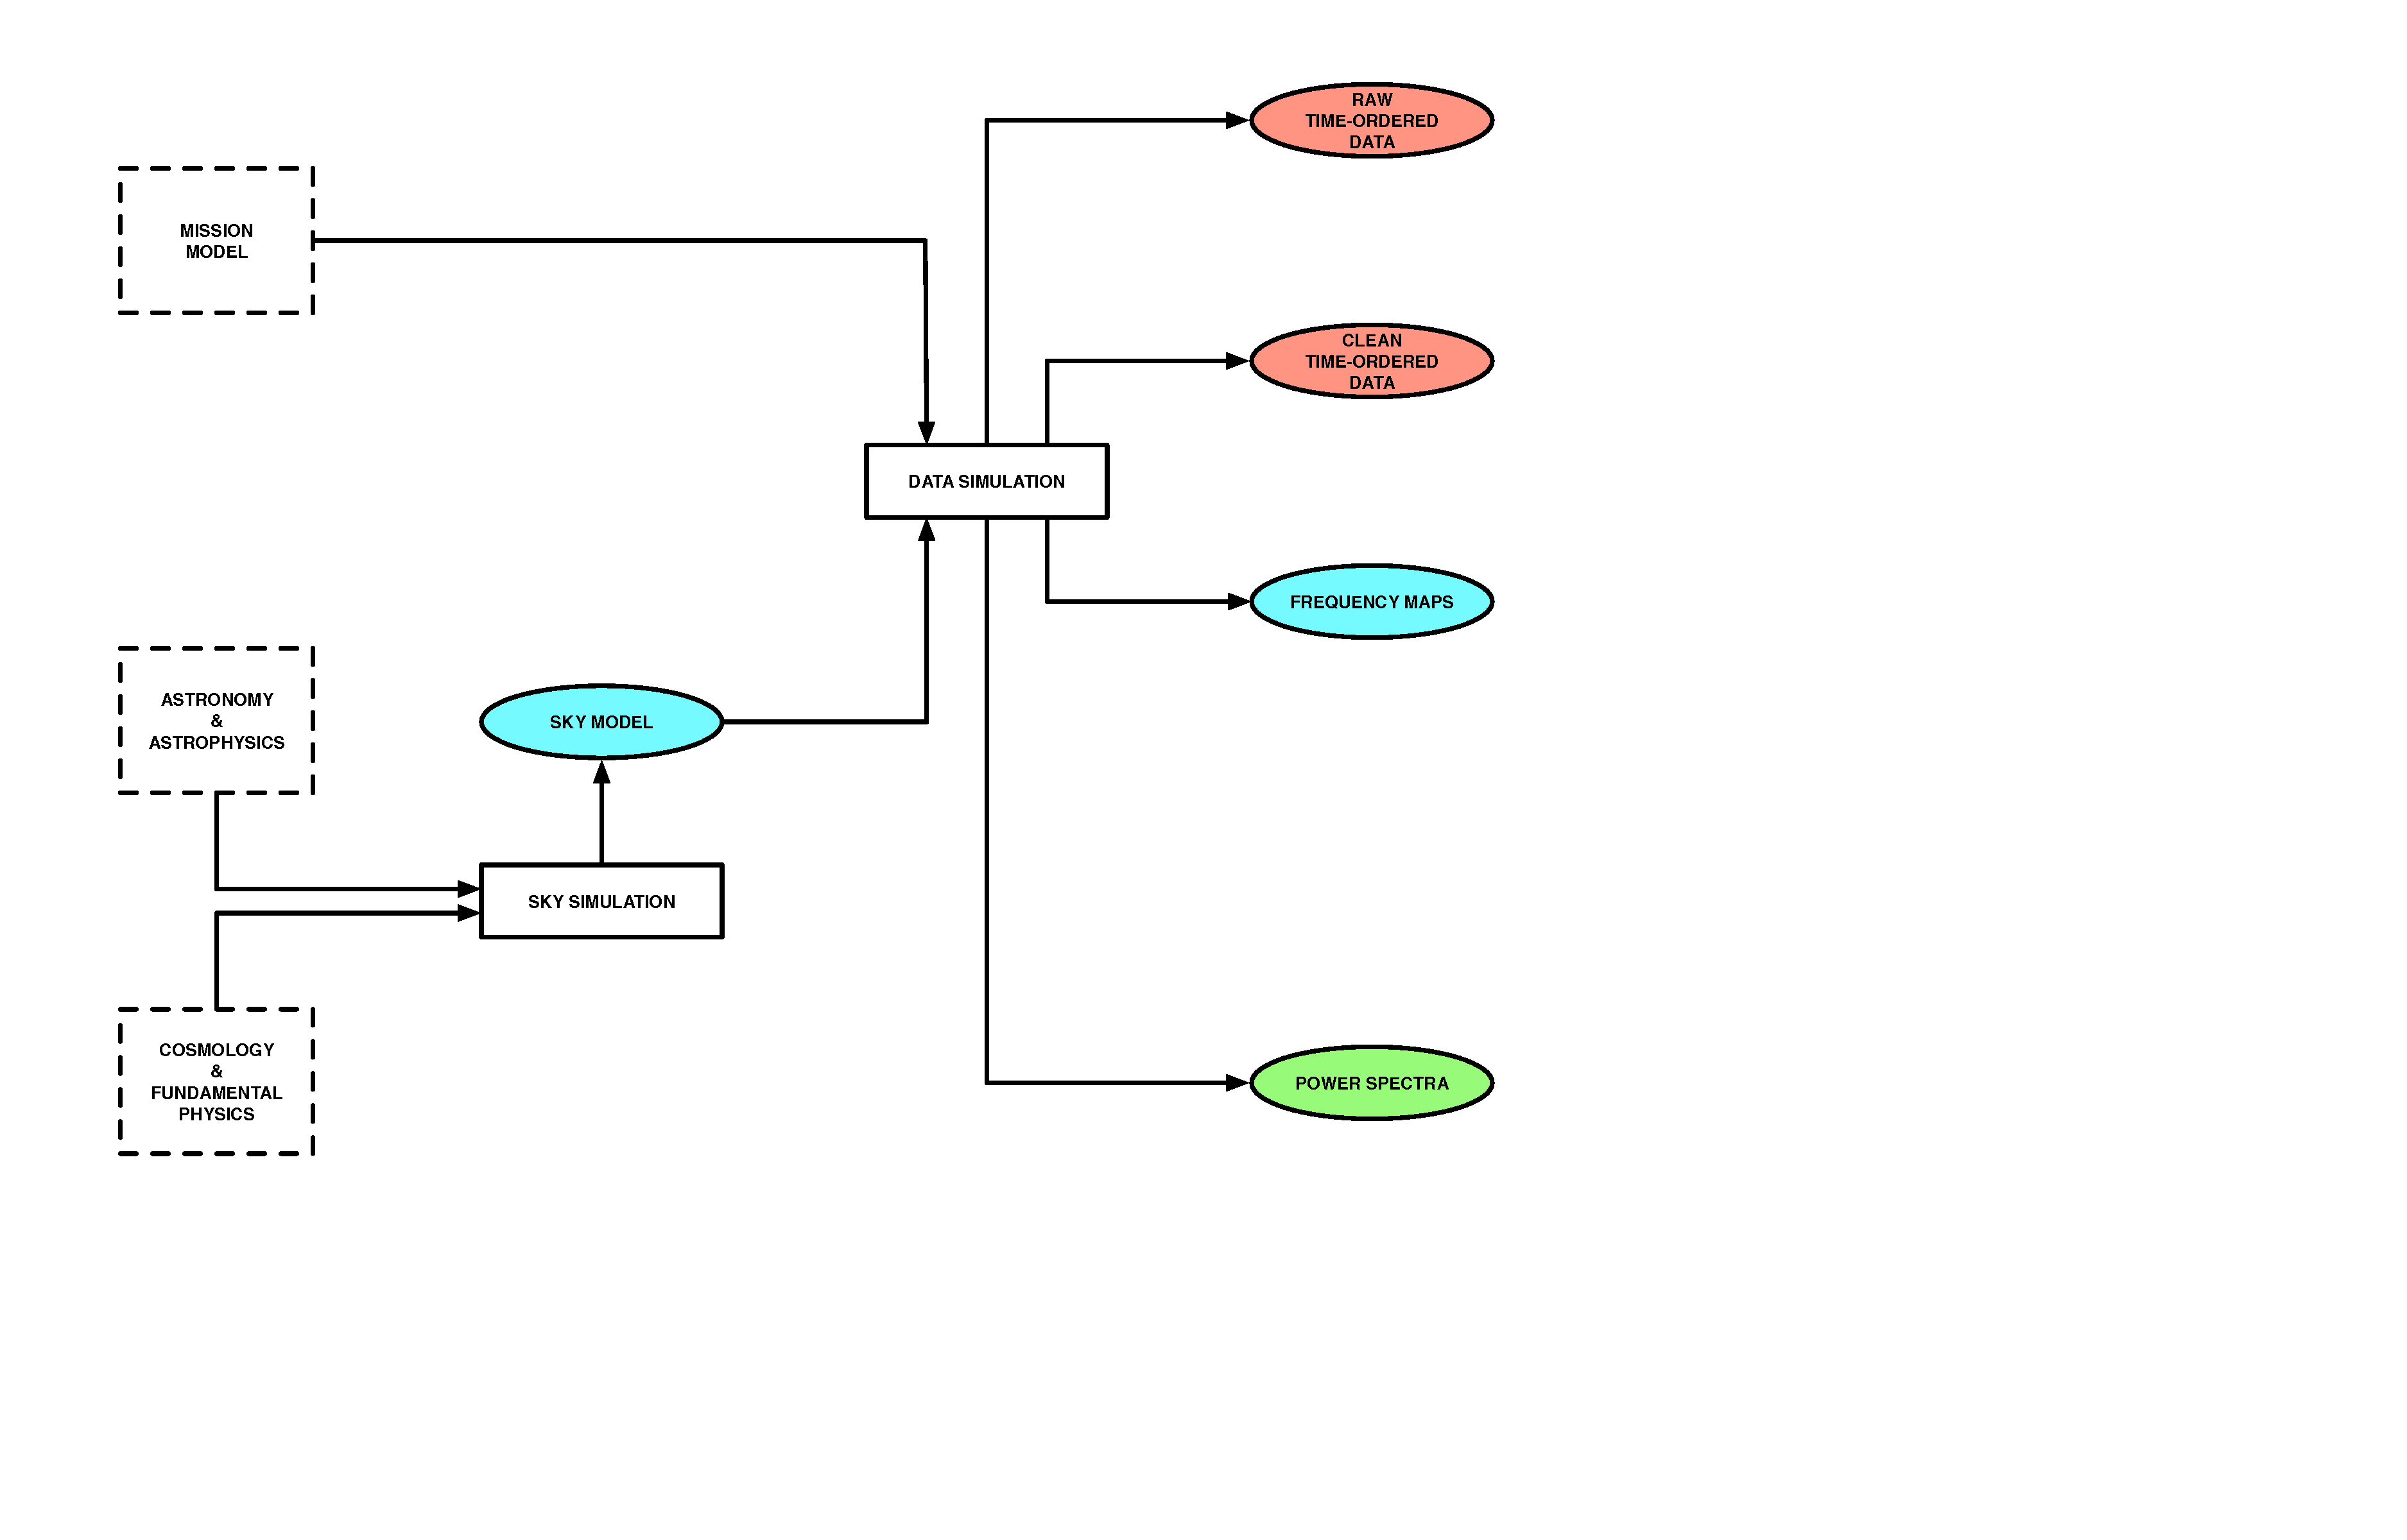
\includegraphics[width=0.5\textwidth]{Analysis/sim}
\caption{The CMB simulation pipeline}
\label{default}

\end{figure}

\newpage

\subsection{Coupling Simulation and Data Analysis}

The overall simulation and data analysis pipeline runs both as a top-down data reduction and a wrap-around refinement of mission and sky characterization and modeling.

It can be subdivided into 5 blocks based on the challenges faced and expertise required to address them.

\begin{figure}[htbp]
\centering
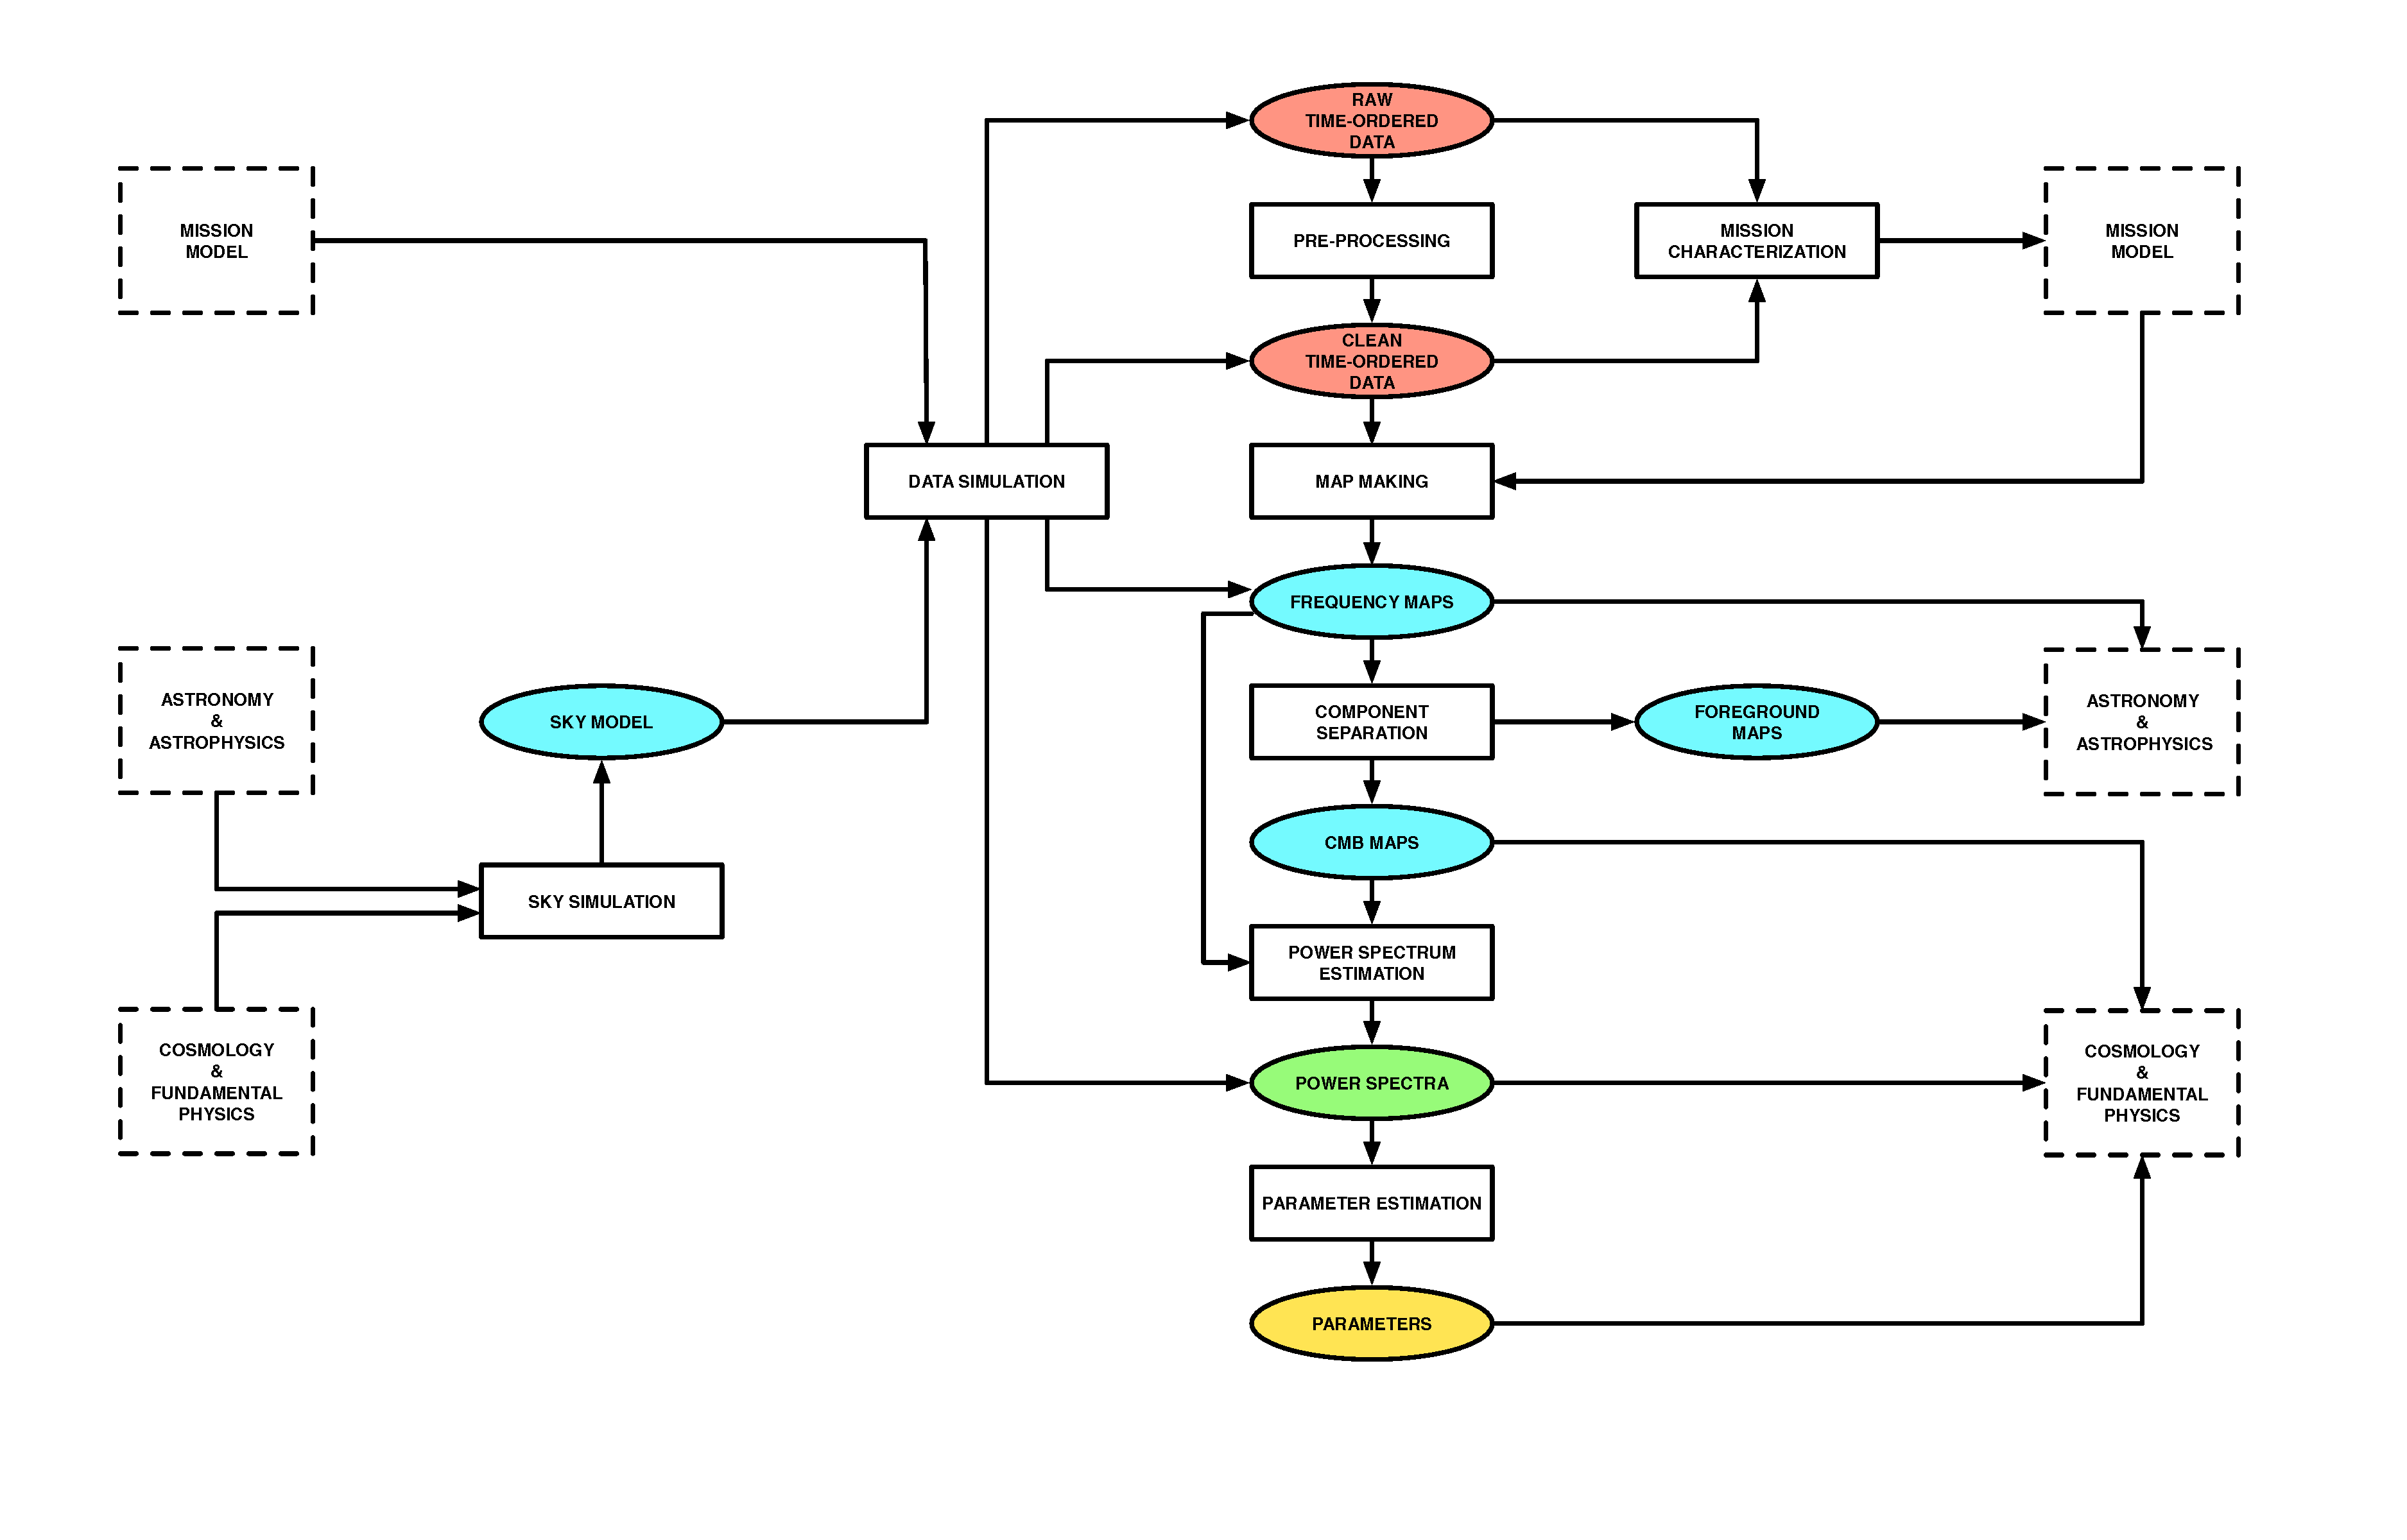
\includegraphics[width=1\textwidth]{Analysis/simda}
\caption{The full CMB simulation/data analysis pipeline}
\label{default}

\end{figure}

\newpage

\input Analysis/forecasting.tex

\newpage

\input Analysis/sky_modeling.tex

\newpage

\input Analysis/tod_processing.tex

\newpage

\input Analysis/component_separation.tex

\newpage

\input Analysis/statistics_parameters.tex

\newpage

%\bibliography{cmbs4}

%%
%% Populate the .bib file with entries from SPIRES Bibtex (preferred)
%% or ADS Bibtex (if no SPIRES entry).
%%  SPIRES will also supply the CITATION line information; please include it.
%%


